\documentclass[tikz]{standalone}
\usepackage{pgfplots}

\pgfplotsset{compat=newest}
\pgfplotsset{
    yticklabel style={
        /pgf/number format/fixed,
        /pgf/number format/precision=2
    },
    scaled y ticks=false
}

\begin{document}
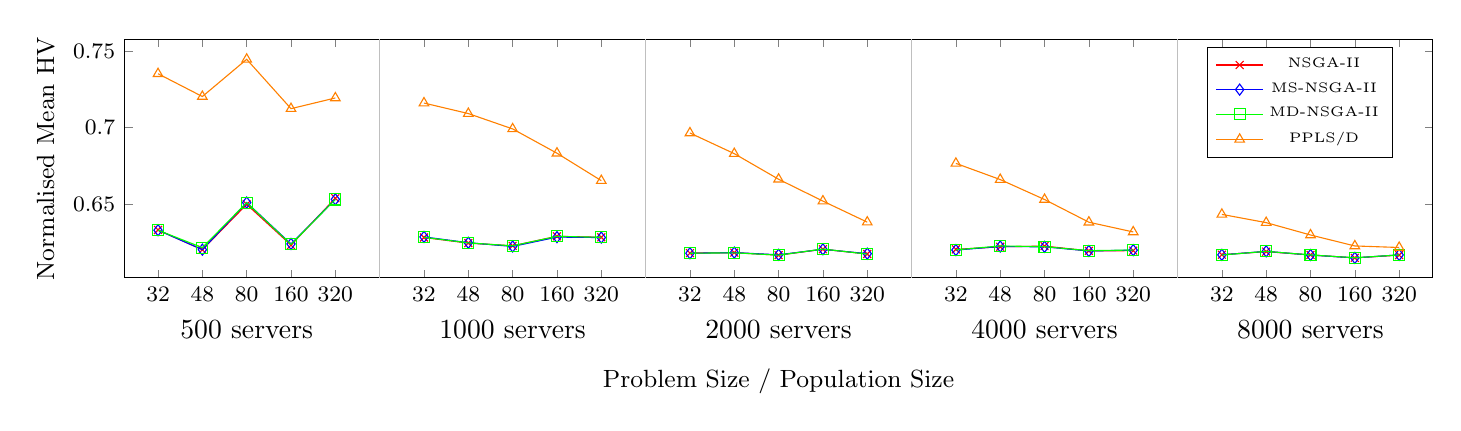
\begin{tikzpicture}

    \begin{axis}[
        footnotesize,
        max space between ticks=20pt,
        width=1.5\textwidth,
        height=0.38\textwidth,
        try min ticks=5,
        xtick=data,
        xticklabels={32, 48, 80, 160, 320, 32, 48, 80, 160, 320, 32, 48, 80, 160, 320, 32, 48, 80, 160, 320, 32, 48, 80, 160, 320},
        extra x ticks={5,11,17,23},
        extra x tick labels={},
        extra x tick style={
            grid=major,
            major tick length=0pt,
        },
        xlabel={Problem Size / Population Size},
        ylabel={Normalised Mean HV},
        xlabel style={
            yshift=-4ex,
        },
        enlarge x limits={abs=0.75},
        legend pos=north east,
        legend entries={
            {NSGA-II},
            {MS-NSGA-II},
            {MD-NSGA-II},
            {PPLS/D},
        },
        clip mode=individual,
        legend style={font=\tiny},
    ]

    \addplot[
        mark=x,
        color=red
    ] table[
        x expr=\coordindex,
        y=PS
    ]{
        HV PS
        32 0.63291
        48 0.61998
        80 0.64972
        160 0.62302
        320 0.65376
        {} {}
        
        32 0.62796
        48 0.62431
        80 0.62252
        160 0.62876
        320 0.62812
        {} {}
        
        32 0.61775
        48 0.61802
        80 0.61638
        160 0.62028
        320 0.61715
        {} {}
        
        32 0.62019
        48 0.62188
        80 0.62233
        160 0.61919
        320 0.61935
        {} {}
        
        32 0.6167
        48 0.61871
        80 0.61653
        160 0.61461
        320 0.61642
        {} {}        
    };

    \addplot[
        mark=diamond,
        color=blue
    ] table[
        x expr=\coordindex,
        y=PS
    ]{
        HV PS
        32 0.63278
        48 0.61999
        80 0.65089
        160 0.62376
        320 0.65302
        {} {}
        
        32 0.62836
        48 0.62455
        80 0.6221
        160 0.62824
        320 0.62794
        {} {}
        
        32 0.61764
        48 0.61807
        80 0.61664
        160 0.62024
        320 0.61735
        {} {}
        
        32 0.61973
        48 0.62208
        80 0.62187
        160 0.61913
        320 0.6197
        {} {}
        
        32 0.61661
        48 0.61889
        80 0.61647
        160 0.61461
        320 0.61658
        {} {}        
    };

    \addplot[
        mark=square,
        color=green
    ] table[
        x expr=\coordindex,
        y=PS
    ]{
        HV PS
        32 0.63276
        48 0.6213
        80 0.65084
        160 0.62345
        320 0.65294
        {} {}
        
        32 0.62812
        48 0.62444
        80 0.6225
        160 0.62872
        320 0.62809
        {} {}
        
        32 0.61766
        48 0.61793
        80 0.61641
        160 0.6204
        320 0.61709
        {} {}
        
        32 0.61988
        48 0.62243
        80 0.62195
        160 0.61934
        320 0.61975
        {} {}
        
        32 0.61649
        48 0.61888
        80 0.61654
        160 0.61468
        320 0.61654
        {} {}               
    };

    \addplot[
        mark=triangle,
        color=orange
    ] table[
        x expr=\coordindex,
        y=PS
    ]{
        HV PS
        32 0.73541
        48 0.72046
        80 0.74488
        160 0.7125
        320 0.71952
        {} {}
        
        32 0.71619
        48 0.70929
        80 0.69921
        160 0.68328
        320 0.66527
        {} {}
        
        32 0.69654
        48 0.68299
        80 0.6662
        160 0.65186
        320 0.63805
        {} {}
        
        32 0.6766
        48 0.66599
        80 0.6529
        160 0.63801
        320 0.63161
        {} {}
        
        32 0.64314
        48 0.63773
        80 0.62962
        160 0.62243
        320 0.62142
        {} {}          
    };

    \begin{scope}[
        every label/.append style={
            label distance=2ex,
        },
    ]
        \node [label=below:500 servers]
            at (axis cs:2,\pgfkeysvalueof{/pgfplots/ymin}) {};
        \node [label=below:1000 servers]
            at (axis cs:8,\pgfkeysvalueof{/pgfplots/ymin}) {};
        \node [label=below:2000 servers]
            at (axis cs:14,\pgfkeysvalueof{/pgfplots/ymin}) {};
        \node [label=below:4000 servers]
            at (axis cs:20,\pgfkeysvalueof{/pgfplots/ymin}) {};
        \node [label=below:8000 servers]
            at (axis cs:26,\pgfkeysvalueof{/pgfplots/ymin}) {};
    \end{scope}
    \end{axis}
\end{tikzpicture}
\end{document}